% \documentclass{report}
\documentclass[12pt, a4paper]{article}
\usepackage{anysize}
\usepackage[centertags]{amsmath}
\usepackage{amsfonts,amssymb,amsthm}
\usepackage{graphicx}
\usepackage{natbib}
\usepackage{url}
\usepackage{wrapfig}
\usepackage{pbox}
\usepackage{a4wide}
\usepackage{graphicx}
\usepackage{amsmath}

\usepackage{listings}
\usepackage{minted}
\usemintedstyle{borland}



\pagenumbering{gobble}

\title{ \textbf{SAFE: Smart Authenticated Fast Exams for Student Evaluation in Classrooms} \\
\vspace{1cm}  \normalsize{M.Tech Project Stage 1 Report} \vspace{1cm} \\
\textit{Submitted in partial fulfillment of the requirements} \\ \textit{for the degree of}  \\ \vspace{1cm} \textbf{Master of Technology} \\ \vspace{1cm} by }
\author{ \textbf{Kurien Zacharia}  \\ 
\vspace{1.5cm}
\textbf{Roll No: 143059002 }}

\begin{document}


 
%\today
\maketitle
\newpage

\newpage
\pagenumbering{arabic}
% \pagenumbering{roman}
\pagestyle{plain}

\begin{abstract}

SAFE is a tool that enables continuous assessment in the form of regular/weekly quizzes in classes. SAFE is based on a BYOD (bring your own device) model that leverages student smartphones to conduct auto-graded, cheating-free exams in a proctored class room setting. SAFE has 3 components: a smartphone app, a web server and WiFi infrastructure to enable app-server communication. The platform has so far been used in 130+ in class quizzes across 9 courses. It was also used to conduct a high stake admission test for a Master’s program in Computer Science.\\

The currently used PHP based server and Android app was initially developed as proof of concept and later expanded to include more features and bug fixes as more people started using the platform. Statistics for quizzes was added to know how students performed in the quiz overall as well as question wise statistics on how many students answered correctly, incorrectly and did not attempt. This feature allows the instructor to know the overall performance of the students and spend more time on the topics that had bad performance. Adding support for code sinppets in the question text was another requirement that was implemented. There was also a requirement for generating a print view of the questions with or without the answers so that instructors could conduct a written quiz parallely, or discuss the questions at a later point of time. \\

As time progressed it became evident that a complete rewrite of the code was required in order to make the code modular, scalable, maintainable and to improve performance. After cosiderable research it was decided to use python based Django framework for the backend, along with PostgreSQL database and Celery for asynchronous tasks. The Android app was also rewritten for better code maintainability and performance. During the time of starting of the project both the Django server and Android app rewrite had just been completed with the bare minimum features to start testing. The first major task was to properly test the newly written code and fix any bugs that was found out in the process. \\

Once the app was stable the next task was to create a docker container to deploy the server in both production and development modes. Prior to this the time required to setup the SAFE server on a fresh machine was around 4 hours. By creating a docker container with all the requirements inside it, the time required for setting up the server on a machine came down to 30 minutes (human intervention is required only in the initial 5 minutes, rest of 25 minutes are taken for downloading of the required software and their installation) \\
   
It was found that many instructors using the platform for the first time had difficulty in understanding the platforms and setting up course / quiz by themselves. There a new UI was prototyped with the latest UI / UX best practices and patterns, to make the system more intuitive and easier to use.
\end{abstract}

\clearpage
\section*{\center\LARGE{Acknowledgement}}

  My sincere thanks to \textbf{Prof.Kameswari Chebrolu} and \textbf{Prof.Bhaskar Raman} for their guidance and supervision
  which served to improve each step of the project. I would also like to thank the department and the office staff for their support and help. Last, but not the least, I would like to thank all my friends and family for their moral support.
 


% Table of Contents
\clearpage
\tableofcontents

\clearpage
\section{Introduction} 
\hspace{0.5cm} 
  
Technology can be used as an aid in improving the quality of education. SAFE can be used to conduct auto-graded, cheating-free exam in a proctored class room setting. This allows the instructor to immediately assess if the students have understood the content.

The current version of SAFE which is being used was created as a proof of concept and later expanded to include the feature requests of the users. But as more people started using SAFE it became evident that a complete rewrite of the App is required to make the code improve performance, scalable and maintainable. The major focus of the Stage 1 project is to implement any critical feature requests / bug fixes in the old version of the App and to stabilize and complete the coding of the new version.
   
\subsection{Work done}

\begin{enumerate}
 
 \item \textbf{Old SAFE Version}
 \begin{itemize}
  \item Create and quiz and questions statistics page
  \item Code snippet and indentation support in question
  \item Create a print ready view of the questions with or without answers
  \item Instructor profile page
  \item Other minor requirements - Reasons list page, bug fixes
  
 \end{itemize}

 \item \textbf{New SAFE Version}
 \begin{itemize}
  \item Thorough testing of the new SAFE Server and App and stabilize the code
  \item Create docker containers for production and development version of the SAFE Server
  \item Create New frontend for the SAFE server which is intuitive and easy to use
 \end{itemize}

\end{enumerate}

\clearpage
\section{Quiz Statistics} 
\hspace{0.5cm} 
    
   
\subsection{Problem statement}
	Create a statistics page per quiz that shows the following statistics
	\begin{enumerate}
	    \item Shows mark distribution of the quiz as a Cumulative Distributive Function (CDF)
	    \item Show the statistics per question of number of students who have answers the question correctly, incorrectly and did not attempt.
		\item Show top 5 answers per questions and the percentage of students who chose each option
		\item General stats about the quiz such as total number of students, total number of submissions, average marks, total marks
	\end{enumerate}

\subsection{Why do we need this?}
	One of the advantages of conducting in class quizzes using the SAFE platform is the immediate feedback. The instructor can know the performance of the students as soon as the quiz is over. The above mentioned statistics will aid the instructor in judging the overall performance of the students, as well as any questions which the students found particularly difficult, so that more time can be spent on the topics in which the student performance was low 

\subsection{Design}
	Ideally the statistics should be calculated when the quiz ends. But since the old version of SAFE did not have a job subsystem which tracks if the particular quiz has ended or not, we have to calculate the statistics each time the statistics page is loaded. We cache the calculated statistics to avoid re-computation if the quiz is not changed the next time the page is loaded. In the new version of SAFE we have an asynchronous task runner using Celery which takes care of problem, and statistics can be calculated when the quiz ends.

\subsection{Implementation}
	The statistics are calculated by iterating over all the submissions for the given quiz. The format of the submission and different question types are given in the table

	The logic for calculating different statistics values are as follows

    \begin{enumerate}    
        \item  \textbf{CDF} - Dictionary with key as floor of marks and value as the count of students who have obtained that mark
	    \item  \textbf{Average Marks} - Calculate sum of marks while iterating through the submissions and take average
	    \item  \textbf{Question Stats} - For each question (response) inside a submission increment the count of the corresponding question depending on whether its correct, wrong or not answered	
	    \item  \textbf{Answer Statistics}
	    \begin{itemize}
	        \item For Single Correct answer question we maintain the count of students who chose each option
		    \item For other question types we find the top 5 answers and their counts using priority queue with a comma concatenated string of answers (in case of multiple answers) as the key and the count as the priority
		\end{itemize}
	\end{enumerate}

	Once the statistics are calculated we save it into the statistics table. This table has a field which stores the timestamp of when the quiz is evaluated when the stats were last calculated. This enables to check if the quiz has been modified and if the statistics needs to be recalculated
	
	On the frontend side the graphs are drawn using morris chart javascript chart library

    \begin{center}
    Listing 1 : Representation of different types of questions
    \end{center}
	
    \inputminted{json}{code/question-type.json}

\subsection{Screenshots}
    \begin{figure}[h!]
    \begin{center}
    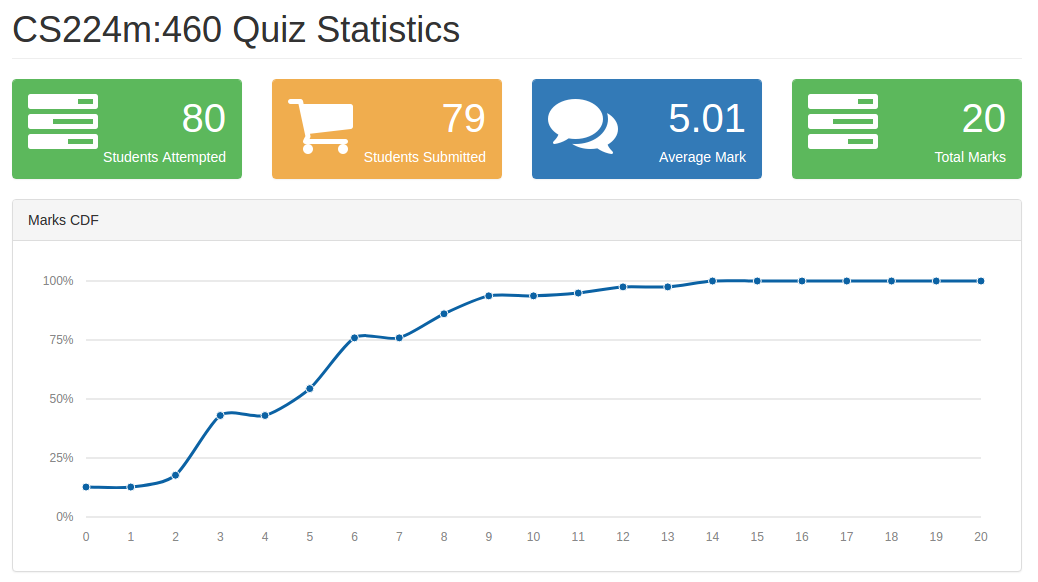
\includegraphics[scale=.4]{diagrams/quiz_stat_1.png} 
    \vspace{1cm}
    \caption{Quiz Statistics Page}
    \end{center}
    \end{figure}
    
    \begin{figure}[h!]
    \begin{center}
    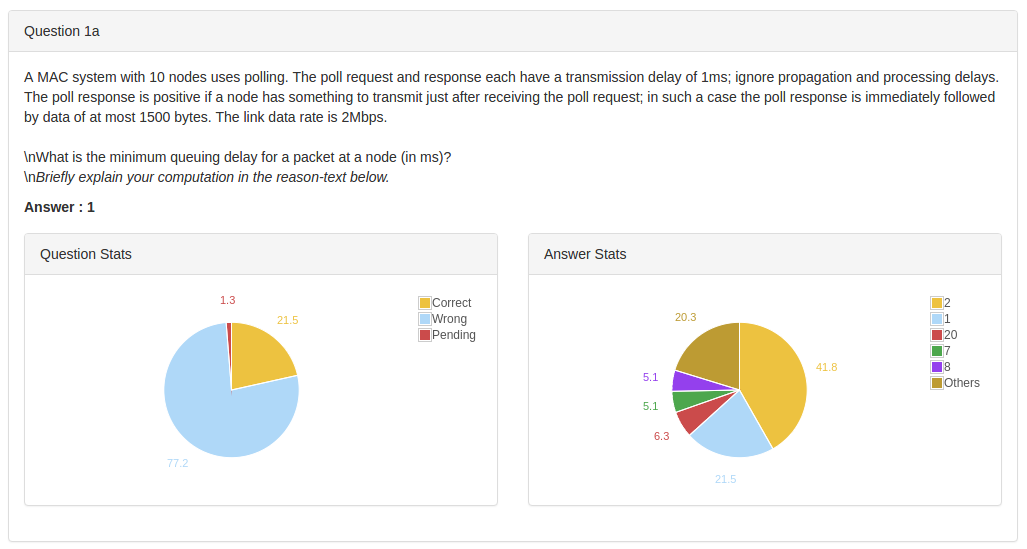
\includegraphics[scale=.4]{diagrams/quiz-stat-2.png} 
    \vspace{1cm}
    \caption{Question statistics}
    \end{center}
    \end{figure}

\clearpage
\section{Code Snippet and Indentation Support} 
\hspace{0.5cm} 
    
   
\subsection{Problem statement}
	Support indentation and code blocks in question text

\subsection{Why do we need this?}
	Many CS courses requires code snippets to be included in the questions. Without proper indentation and code blocks support reading of code snippets is very difficult especially on a mobile device 

\subsection{Design}
	Since the app displays the question text inside a web view, $\langle pre \rangle$ tags can be used to provide indentation support for code blocks. 

\subsection{Implementation}
	Support for $\langle pre \rangle$ tags is implemented by modifications in the following places

    \begin{enumerate}
        \item Change in quiz template parsing to support $\langle pre \rangle$ tags\\ 
        The normal logic during parsing of the the quiz template file is to trim all the extra spaces in each line. But for the contents inside the pre tag we want to keep the contents as such without trimming the spaces. We parse the quiz template file line by line and we use a flag to decide if the current line needs to be trimmed. The flag is set when a '$\langle pre \rangle$' tag is seen and unset when the '$\langle /pre \rangle$' tag is seen
        \item Add CSS styles for $\langle pre \rangle$ tag in the frontend, and in the android app\\
        CSS styes are added to make the code block look better, and use monospace fonts
    \end{enumerate}	


\clearpage
\section{Other Requirements} 
\hspace{0.5cm} 

\subsection{Quiz Print View}
\subsubsection{Problem Statement}
	Generate a printable view of quiz with or without answers

\subsubsection{Why Do we need this?}
	Many times its necessary to discuss the questions with the students after the quiz along with the correct answers. There wasn't a simple view which showed all the questions along with their answers in a simple format. Also for some quizzes there were students who wanted to take the quiz offline. A printable page with just the questions would allow the instructor to conduct the quiz using the app and offline simultaneously.

\subsubsection{Implementation}
	Displaying of question has two parts - the question text and the answers. Getting the Question text is straight forward and is directly obtained from the database field. Answers depends on the type of question

    \begin{itemize}
        \item Integer question - Directly print the answer
	    \item Single and multiple answer question - Print the options and put a tick symbol on the answer
	    \item Fill in the blanks question - List all possible answers separated by comma
	    \item Floating point type question - Print the possible range of answers in the form of <lower bound> to <upper bound>
	\end{itemize}

\begin{figure}[h!]
\begin{center}
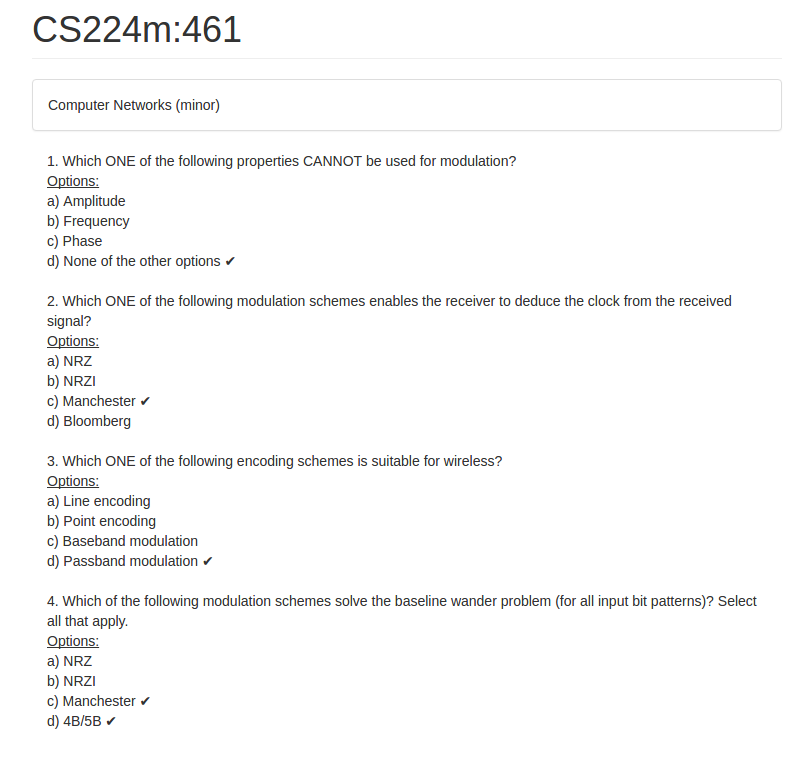
\includegraphics[scale=.4]{diagrams/print-view} 
\vspace{1cm}
\caption{Print View of Quiz}
\end{center}
\end{figure}

\subsection{Instructor Profile Page}
\subsubsection{Problem Statement}
	Create a My Account page for instructor which allows them to change their personal details and passowrd

\subsubsection{Implementation}
	Saving of personal details is a direct update to the database entry. Password is hashed using BCRYPT hashing method and then saved to the database. 

\subsection{Reason texts list page}
\subsubsection{Problem Statement}
	Create a page to list all reason texts given by students grouped by the question

\subsubsection{Why do we need this?}
	Reason text is a feature using which students can explain the reason behind their answer, or how they arrived at their answers. This is userful in many cases where the students needs to be evaluated for his methodoloty of solving the problem or reasoning. Displaying a list of all the reasons texts given by the students along with the Quiz Statistics feature 4allows to instructor to know how and why the students chose a particular answer.

\subsubsection{Implementation}
	We iterate over the submissions for the particular quiz and create a dictionary with the key as the question_id and the value as a list of reasons given for the particular question	

\begin{figure}[h!]
\begin{center}
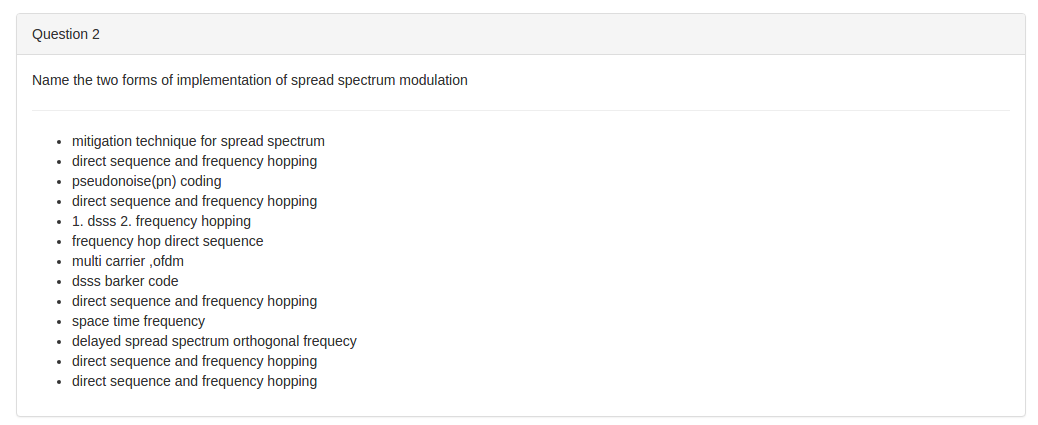
\includegraphics[scale=.4]{diagrams/reasons-list} 
\vspace{1cm}
\caption{Reasons list page}
\end{center}
\end{figure}

\clearpage
\section{Stabilize new SAFE code} 
\hspace{0.5cm} 

\subsection{Problem Statement}
	Thourough testing of the New SAFE Server and App

\subsection{Why do we need this?}
	The rewritten SAFE server and App was not tested rigorously. This led to many bugs some of which were critical to taking a test. There was a need to stabilize the code first before adding new features

\subsection{Design}
	A testing matrix was created with all the current features in the platform. This ensured that not feature was left untested and also features worked with each other.

\subsection{Implementation}
	All the features were tested independently. Also all the critical feautres were tested with each other. 19 critical bugs were found along with other minor bugs and were fixed. Table shows the list of the critical bugs, the steps to reproduce them and the cause of the bug. Some of the bugs were multithreaded bugs which were difficult to reproduce and debug. A lot of effort was put to ensure that the code is stabilised before addition of new features.\\

    List of bugs fixed
    
    \begin{itemize}
        \item \textbf{Build organization list cache automatically} - Organization list cache is not populated automatically. The only way to populate the organization list cache is to run the management command
        
        \item \textbf{Submission evaluation atomic requests bug} - Atomic Requests causes celery to not see the response written to the database
        
        \item \textbf{Quiz Live Dashboard Data table page change time stamp not correct} - Moment.js which formats the timestamp is not called when the datatable page is changed
        
        \item \textbf{Marks after evaluation comes as 2/1 randomly} - When the same option is repeated it caused the evaluation to add marks twice since there is no ID associated with the option
        
        \item \textbf{Server not sending submitted response in api for previous submission} - Server is sending the response as a separate dictionary, it should ideally send the response, marks obtained and reason text along with the question modules
        
        \item \textbf{Quiz cache population bug due to atomic request} - Atomic Requests cases celery to not see the new questions written to the database
        
        \item \textbf{Reload organization list on Server URL change} - Organization list should be refreshed when the server url is changed
        
        \item \textbf{Quiz ID input does not submit when enter on keyboard is pressed} - IME action for the EditText is not defined
        
        \item \textbf{Multiple Choice Question answers data type is Array of Int instead of Int} - Answer field is an int, not an array of int
        
        \item \textbf{If MCQ has repeated options only once of them is displayed} - WebView cache key for the options is the same, which causes the same web view to be reused for all the options. So only the last one is shown. Others are reused
        
        \item \textbf{LoginToken not reset during activity creation in LoginActivity} - AuthToken from the previous server is not cleared when the server URL is changed. This results in invalid token error from the new server
        
        \item \textbf{Periodic submissions fail randomly} - Websockets do not run in developement mode
        
        \item \textbf{Previous submission choices are changeable} - The submitted response field was not populated from the JSON returned from the server
        
        \item \textbf{Infinite Quiz implementation is broken} - Bug in parsing logic of server response
    
    \end{itemize}
    
\begin{figure}[h!]
\begin{center}
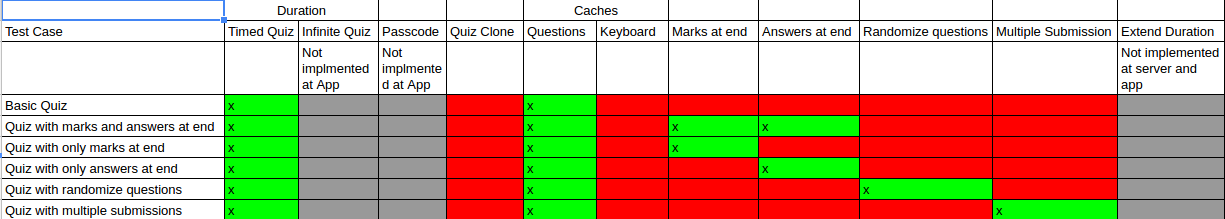
\includegraphics[scale=.4]{diagrams/test-matrix-1} 
\vspace{1cm}
\caption{Test Matrix of Different Quiz Settings}
\end{center}
\end{figure}


\begin{figure}[h!]
\begin{center}
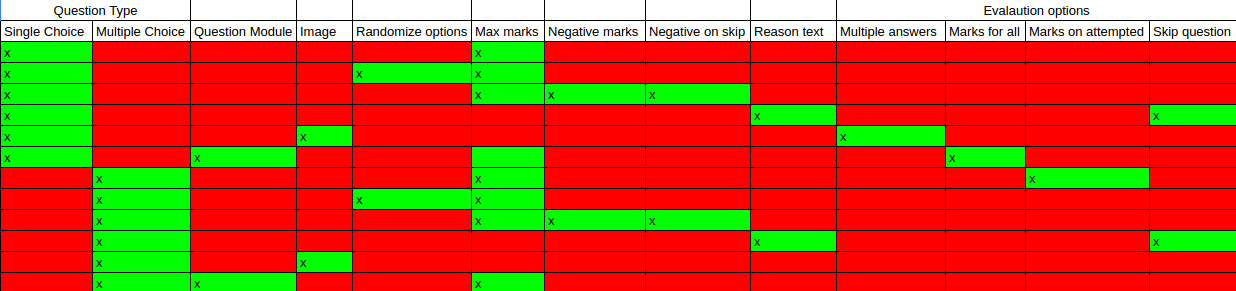
\includegraphics[scale=.4]{diagrams/test-matrix-2} 
\vspace{1cm}
\caption{Test Matrix of Question Types}
\end{center}
\end{figure}

\clearpage
\section{Docker Containers for SAFE} 
\hspace{0.5cm} 


\subsection{Problem Statement}
	Create docker containers for the production and developement setup of SAFE

\subsection{Why do we need this?}
	Installating and configuring all the requirements to run SAFE took around 3-4 hours. On top of that on production servers there were version conflicts for some of the requirements making the setup of SAFE very complicated and error prone. 

\subsection{Design}
	Docker containers unlike VM's are not full operating systems. Instead only the libraries and settings required for the software to work are needed. There are much lighter than VM's and has almost bare metal performance. Containers are isolated from the host and with other containers. So docker container run same everwhere irrespective of where it is deployed.\\

	Once Docker containers are setup up SAFE can be installed and configured with just one command reducing the time taken to approximately 30 minutes

\subsection{Implementation}
	SAFE requires two different setups for the production mode and developement mode. Therefore two docker configurations was created for them. The docker setup for SAFE includes the following containers

    \begin{itemize}
        \item Postgres Container - Runs PostgreSQL version 9.5
        \item Postgres Data Container - This container stores the postgres data files. This is a requirement of Docker containers to persist the database to the disk between runs of containers
        \item Redis Container - Runs redis version 3.2 (used as a cache and broker for celery)
        \item Web Container - This is a container created from scratch and has all the necessary web server related packages like nginx, django, nodejs, uwsgi etc.
	\end{itemize}
 
 	

\clearpage
\section{Quiz Upload / Download From XML File} 
\hspace{0.5cm} 


\subsection{Problem Statement}
	Instructor should be able to Upload / Download quiz as XML file

\subsection{Why do we need this?}
	Even though SAFE provides an intuitive UI to create and edit quiz, sometimes instructors will have a template of their quiz and would like to use it as a starting point. Using an xml file as the template instructors can upload the template and then use the UI to make edits in the quiz.\\
	
	XML download also allows to create backups of the quiz

\subsection{Implementation}
	We use the ElementTree library for XML parsing in Python.

    \begin{itemize}
        \item Postgres Container - Runs PostgreSQL version 9.5
        \item Postgres Data Container - This container stores the postgres data files. This is a requirement of Docker containers to persist the database to the disk between runs of containers
        \item Redis Container - Runs redis version 3.2 (used as a cache and broker for celery)
        \item Web Container - This is a container created from scratch and has all the necessary web server related packages like nginx, django, nodejs, uwsgi etc.
	\end{itemize}
 
 	

\clearpage
\section{New Frontend for SAFE Server} 
\hspace{0.5cm} 

\subsection{Problem Statement}
	Create a new frontend for the SAFE server, which is intuitive and easy to use

\subsection{Why do we need this?}
	The current UI/UX of the SAFE server was difficult to understand and use. Also the Industrial Design Centre (IDC) in IIT reviewed SAFE and gave a low Usability score. It was necessary to create a new Frontend which adhered to the common UX patterns and make it easy even for a new user to use the system. 

\subsection{Design}
	Multiple brainstorming sessions were done to identify the pain points in the current Server and how these can be fixed. We have also gone through the UI/UX guidelines of Google and Facebook and made sure the new frontend adhered to these guidelines and best practices. Care was taken to reduce the number of clicks the user has to do to execute some action. Color schemes was also fixed so that there is a uniform look and feel throughout the site.

\subsection{Implementation}
	After much dicussion the following Pages were finalized

    \begin{itemize}
        \item Dashboard - Shows list of currently running quizzes, recent quiz instances and quizzes and courses
	    \item Course page with following subpages
	    \begin{itemize}
	        \item Quizzes page - Shows all the quizzes in the given quiz along with quiz access buttons for frequent actions like running a quiz, editing a quiz etc.
		    \item Settings page - View / Edit Course Settings
	    \end{itemize}
		
	    \item Quiz Page
	    \begin{itemize}
	        \item Questions page - View all the questions in the quiz along with quiz settings
		    \item Quiz edit page - Create / Edit questions in a quiz in a Google forms like interface using drag and drop
		    \item Settings page - View / Edit quiz settings
		    \item Instances - Run new instances of quiz
		    \item Quiz live Dashboard - See live statistics about a running quiz and alerts
		    \item Submissions - Unified page to see both partial submissions and final submissions of different instances. 
		    \item Statistics - Statistics for the quiz
	    \end{itemize}
	\end{itemize}

	A fully working prototype (not linked with the actual server, runs on dummy data, but fully fuctional) was created using a bootstrap based opensource Admin template - AdminLTE along with custom CSS. AngularJS v1.6 was used as the javascript library since it allows quick prototyping for the complex interaction which were required for the new design. After creating the initial prototype we did 4 iterations of usability testing and refinements to ensure that any issues found are fixed.
 
\subsection{Screenshots}

\begin{figure}[h!]
\begin{center}
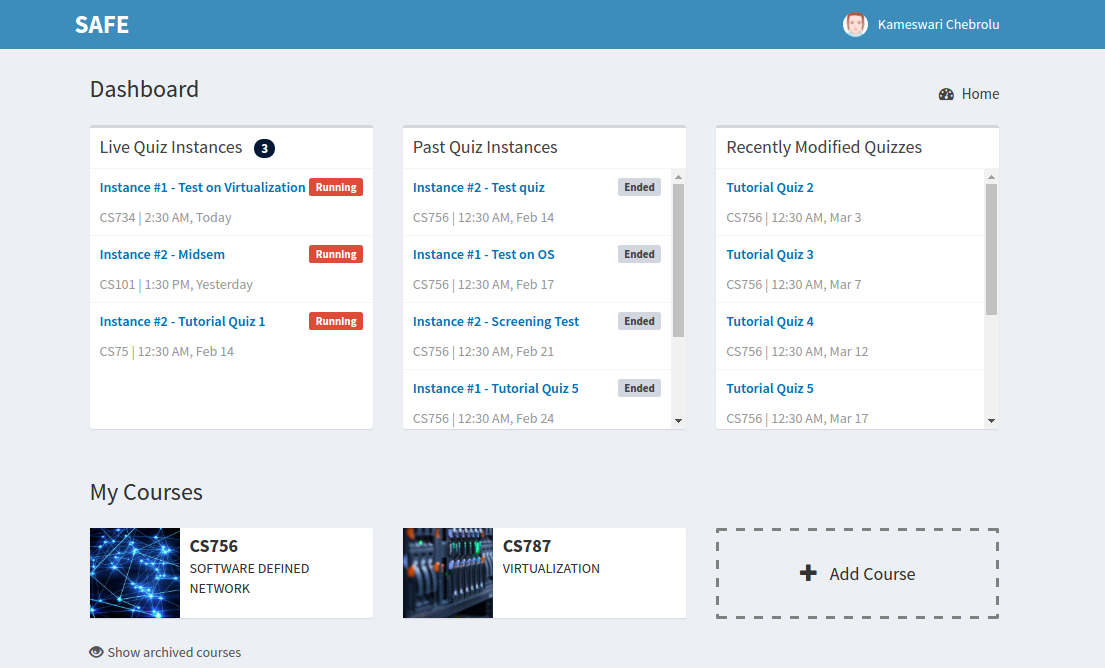
\includegraphics[scale=.4]{diagrams/new-ui-1} 
\vspace{1cm}
\caption{Dashboard Page}
\end{center}
\end{figure}


\begin{figure}[h!]
\begin{center}
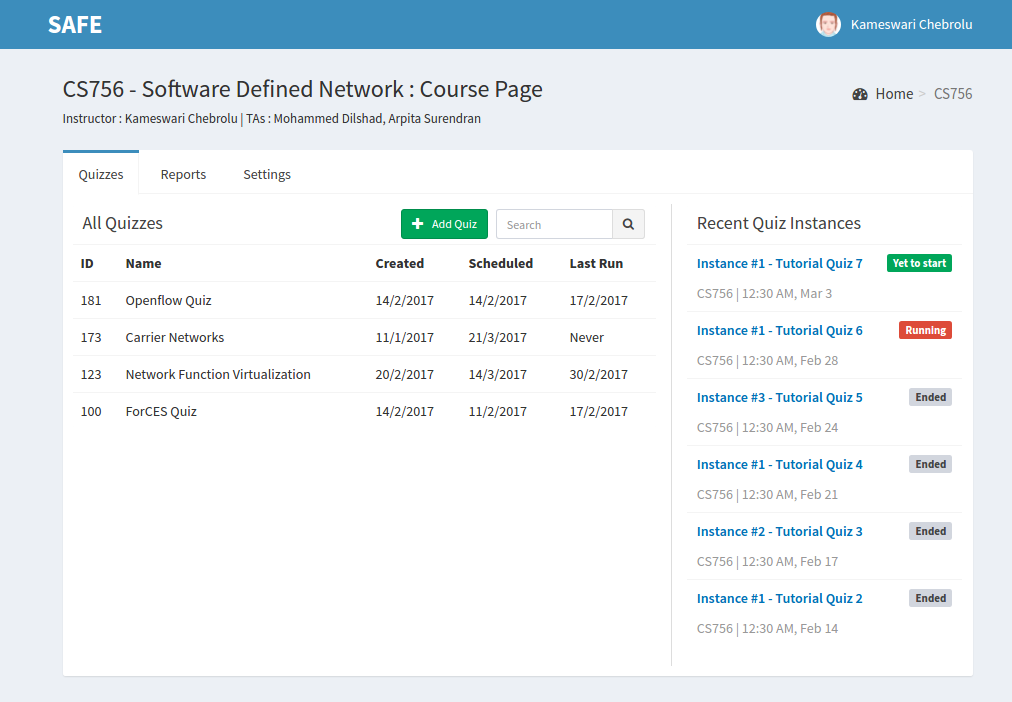
\includegraphics[scale=.35]{diagrams/new-ui-2} 
\caption{Course Page}
\end{center}
\end{figure}

\begin{figure}[h!]
\begin{center}
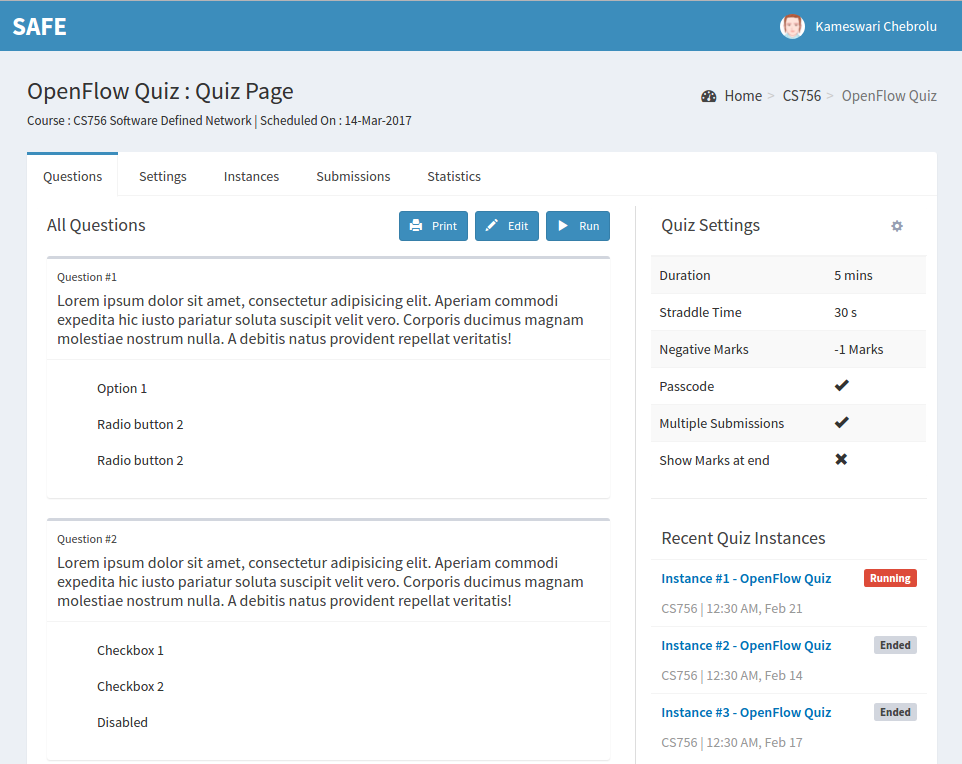
\includegraphics[scale=.35]{diagrams/new-ui-3} 
\caption{Quiz Questions Page}
\end{center}
\end{figure}

\begin{figure}[h!]
\begin{center}
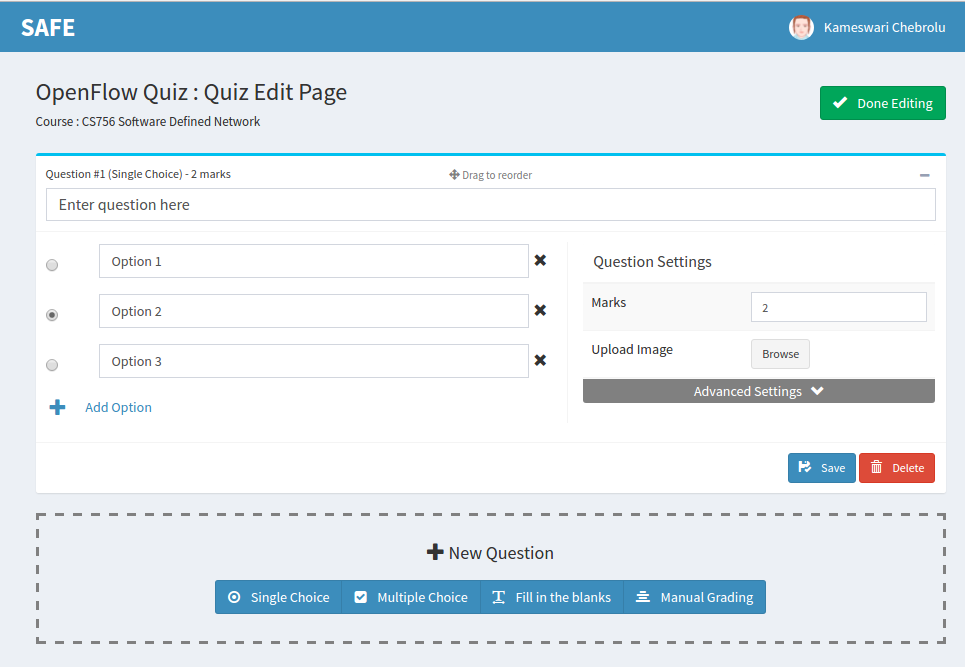
\includegraphics[scale=.4]{diagrams/new-ui-4} 
\caption{Quiz Edit Page}
\end{center}
\end{figure}

\begin{figure}[h!]
\begin{center}
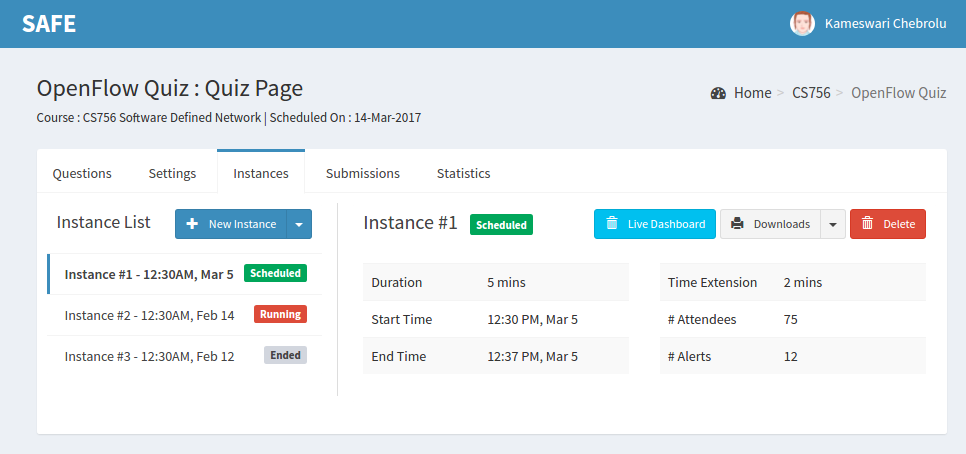
\includegraphics[scale=.4]{diagrams/new-ui-5} 
\caption{Quiz Instances Page}
\end{center}
\end{figure}


 
 
 \section{Futurework}
 
 \begin{itemize}
  \item Code the newly created frontend in Django
  \item Identifying methods for further control of WiFi traffic, and to scale the number of users to use any generic application.
  
 \end{itemize}

\clearpage
\bibliographystyle{plain}
\bibliography{myreferences}


\end{document}

